We work on feature branches, open a pull request to \code{dev}, and later merge \code{dev}
into \code{main}.

\textbf{Tests run on GitHub's machines, not on ours.} \code{tests.yml} runs ruff and pytest
for every push and pull request. The repository is public, so anyone can open a pull request,
and we did not want that code to run on our VMs. The tests use a small local Spark session,
so they need no data. On 23 November \code{ubuntu-latest} changed its default Java and Spark
could no longer write Parquet, so the workflow now pins Java 17, the same as on the VMs.

\textbf{Deploy on merge.} The self-hosted runners only run code that is already merged.
\code{deploy.yml} updates the dev VM on a merge to \code{dev} and the prod VM on a merge to
\code{main} (\code{git pull} and \code{pip install}), so the VMs never run code nobody reviewed.

\textbf{The nightly run.} \code{pipeline.yml} runs at 03:17 UTC on the prod runner, or by hand
for any day on dev or prod. Bronze stays on cron because it needs exact timing, while Silver
and Gold can start a bit late, and in Actions we get logs, history and a red or green status
for free. The first scheduled runs started up to 7.5 hours late; moving from 04:00 to 03:17
helped, because GitHub delays full-hour schedules the most.

\textbf{The run page tells us if the day is good.} At the end the workflow writes a summary
(Bronze runs, Silver rows, Gold status), also after a failure. On prod the run also turns red
with fewer than 270 of 288 valid snapshots: the 20{,}000-row check in Gold alone would let a
half day through.

% Results figure, placed here so the float lands before the Results section.
\begin{figure*}[t]
\centering
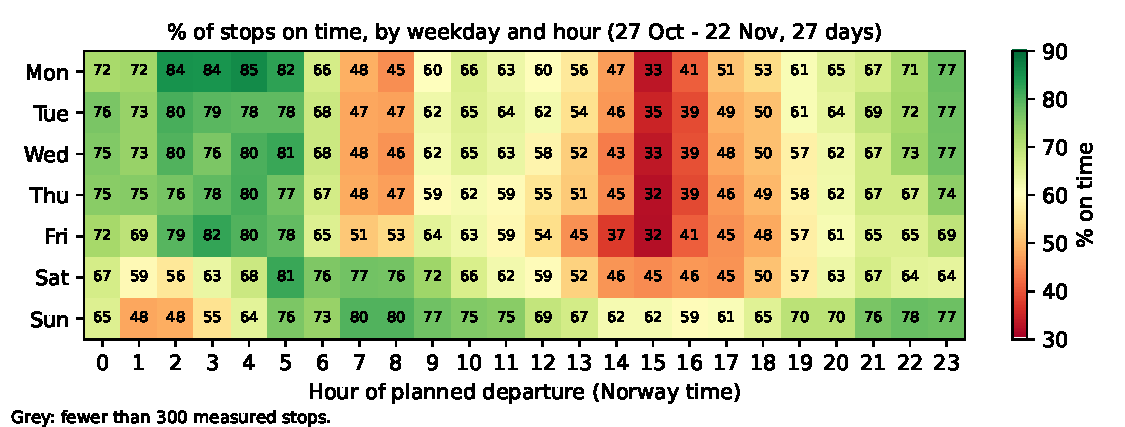
\includegraphics[width=0.85\textwidth]{1_heatmap_weekday_hour.pdf}
\caption{On-time share by weekday and hour of planned departure (Norwegian time).}
\label{fig:heatmap}
\end{figure*}
